\documentclass{article}
\usepackage[english]{babel}
\usepackage[utf8x]{inputenc}
\usepackage{amsmath}
\usepackage{graphicx}
\usepackage{tikz} % Package for drawing

\definecolor{cqcqcq}{rgb}{0.75,0.75,0.75}


\title{12.1 Tests}
\author{chris }
\date{October 2017}

\begin{document}


\noindent BECA / Huson / 12.1 IB Math SL \qquad \qquad Name:\\
24 October 2017
\subsection*{Homework: IB Differential calculus exam problems}

\begin{enumerate}

\item In an arithmetic sequence, $S_{40} =1900$ and $u_{40} =106$. Find the value of $u_1$ and of $d$.

\item Let $f(x)=cos2x$ and $g(x)=ln(3x−5)$.
\begin{enumerate}
\item Find $f ′(x)$.
\item Find $g′(x)$.
\item Let $h(x) = f (x)× g (x)$. Find $h′(x)$.
\end{enumerate}

\item Consider the curve with equation $f(x) = px^2 + qx$, where $p$ and $q$ are constants. The point A(1, 3) lies on the curve. The tangent to the curve at A has gradient 8. Find the value of $p$ and of $q$.

\item A farmer wishes to create a rectangular enclosure, ABCD, of area 525 $m^2$, as shown below.

\begin{figure}[!htbp]
\begin{center}
\begin{tikzpicture}

\draw [thick, -] (-3,3) -- (3,3) node [right] {$C$};
\draw [thick, -] (3,0) -- (-3,0) node [left] {$A$};
\draw [thick, -] (-3,0) -- (-3,3) node [left] {$D$};
\draw [thick, -] (3,3) -- (3,0) node [right] {$B$};

\end{tikzpicture}
\end{center}
\end{figure}

The fencing used for side AB costs \$11 per metre. The fencing for the other three sides costs \$3 per metre. The farmer creates an enclosure so that the cost is a minimum. Find this minimum cost.

\newpage 

\item Let $\displaystyle f(x) = 5cos \frac{\pi}{4} x$ and $g(x) = −0.5x^2 + 5x −8$, for $0 \leq x \leq 9$.
\begin{enumerate}
\item On the same diagram, sketch the graphs of $f$ and $g$.
\item Consider the graph of $f$ . Write down
\begin{enumerate}
\item the x-intercept that lies between $x = 0$ and $x = 3$;
\item the period;
\item the amplitude.
\end{enumerate}
\item Consider the graph of $g$. Write down
\begin{enumerate}
\item the two $x$-intercepts;
\item the equation of the axis of symmetry.
\end{enumerate}
\end{enumerate}

\end{enumerate}


\begin{figure}[!htbp]
\begin{center}
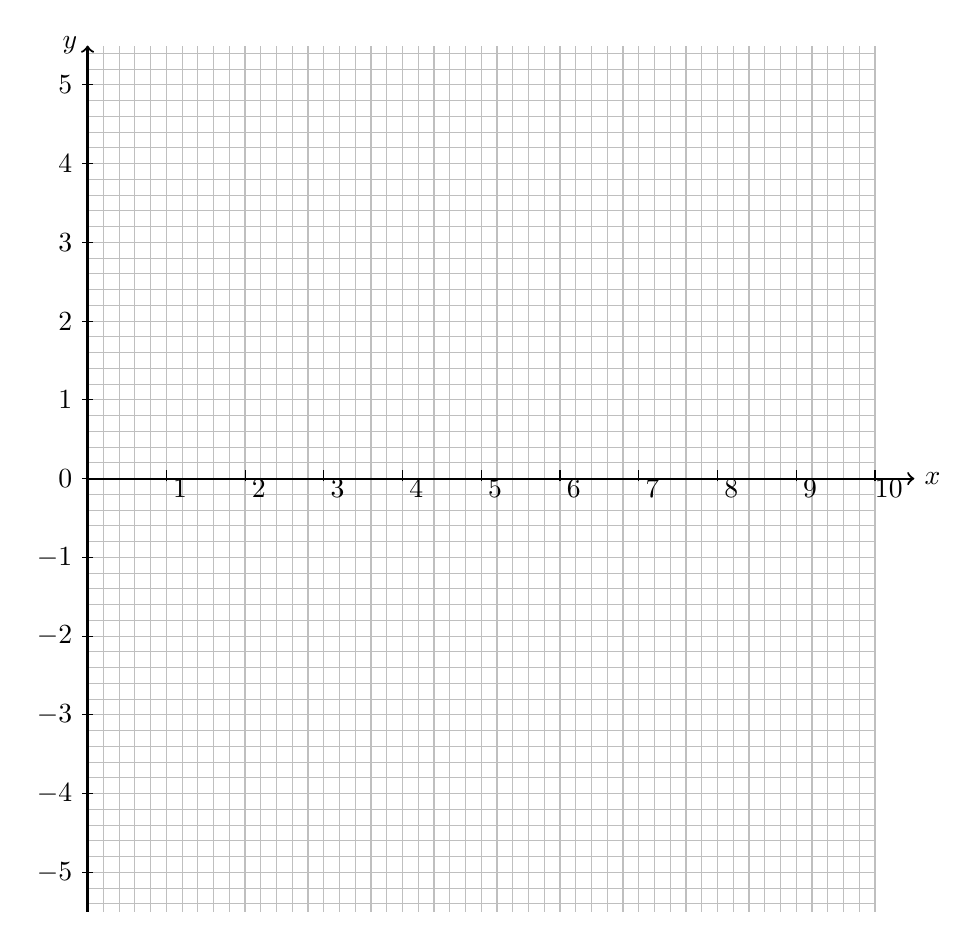
\begin{tikzpicture}

%grid
\draw [color=black,, xstep=1.0cm,ystep=1.0cm] (0,-5.5) grid (10.,5.5);
\draw [color=cqcqcq,, xstep=0.2cm,ystep=0.2cm] (0,-5.5) grid (10.,5.5);

\foreach \x in {,1,2,3,4,5, 6, 7, 8, 9, 10}
\draw[shift={(\x,0)},color=black] (0pt,-1pt) -- (0pt,3pt) node[below]  {$\quad \x$};

\foreach \y in {-5,-4,-3,-2,-1,0,1,2,3,4,5}
\draw[shift={(0,\y)},color=black] (2pt,0pt) -- (-2pt,0pt) node[left]  {$\y$};

\draw [thick, ->] (0,0) -- (10.5,0) node [right] {$x$};
\draw [thick, ->] (0,-5.5) -- (0,5.5) node [left] {$y$};

\end{tikzpicture}
\end{center}
\end{figure}


\end{document}